% --------------------------------------------------------------------------- %
% Poster for the ECCS 2011 Conference about Elementary Dynamic Networks.      %
% --------------------------------------------------------------------------- %
% Created with Brian Amberg's LaTeX Poster Template. Please refer for the     %
% attached README.md file for the details how to compile with `pdflatex`.     %
% --------------------------------------------------------------------------- %
% $LastChangedDate:: 2011-09-11 10:57:12 +0200 (V, 11 szept. 2011)          $ %
% $LastChangedRevision:: 128                                                $ %
% $LastChangedBy:: rlegendi                                                 $ %
% $Id:: poster.tex 128 2011-09-11 08:57:12Z rlegendi                        $ %
% --------------------------------------------------------------------------- %
%\documentclass[apaper,fontscale=0.493,portrait]{baposter} %portrait
\documentclass[a0paper,fontscale=0.4125,landscape]{baposter} %landscape
\usepackage{relsize}		% For \smaller
\usepackage{url}			% For \url
\usepackage{epstopdf}	% Included EPS files automatically converted to PDF to include with pdflatex
\usepackage{booktabs}
\usepackage{subfigure}
\usepackage[export]{adjustbox}
\usepackage{enumitem}
\usepackage{wrapfig}
\usepackage{graphicx}
\usepackage{caption}
\usepackage[sorting=none, citestyle=numeric-comp]{biblatex}
\addbibresource{references.bib}
%\renewcommand*{\bibfont}{\scriptsize}
\renewbibmacro{in:}{}
\usepackage{amsmath}
\usepackage{adjustbox}
\usepackage[font=small,labelfont=bf]{caption}
\usepackage{amssymb}
\usepackage{pbox}

%%% Global Settings %%%%%%%%%%%%%%%%%%%%%%%%%%%%%%%%%%%%%%%%%%%%%%%%%%%%%%%%%%%

\graphicspath{{pix/}}	% Root directory of the pictures
\tracingstats=2			% Enabled LaTeX logging with conditionals

%%% Color Definitions %%%%%%%%%%%%%%%%%%%%%%%%%%%%%%%%%%%%%%%%%%%%%%%%%%%%%%%%%

\definecolor{bordercol}{RGB}{40,40,40}
\definecolor{headercol1}{RGB}{206,215,230}
%\definecolor{headercol2}{RGB}{80,80,80}
\definecolor{headercol2}{RGB}{255,255,255}
\definecolor{headerfontcol}{RGB}{0,88,255}
\definecolor{boxcolor}{RGB}{255,255,255}

%%%%%%%%%%%%%%%%%%%%%%%%%%%%%%%%%%%%%%%%%%%%%%%%%%%%%%%%%%%%%%%%%%%%%%%%%%%%%%%%
%%% Utility functions %%%%%%%%%%%%%%%%%%%%%%%%%%%%%%%%%%%%%%%%%%%%%%%%%%%%%%%%%%

%%% Save space in lists. Use this after the opening of the list %%%%%%%%%%%%%%%%
\newcommand{\compresslist}{
	\setlength{\itemsep}{4pt}
	\setlength{\parskip}{0pt}
	\setlength{\parsep}{0pt}
}

%%%%%%%%%%%%%%%%%%%%%%%%%%%%%%%%%%%%%%%%%%%%%%%%%%%%%%%%%%%%%%%%%%%%%%%%%%%%%%%
%%% Document Start %%%%%%%%%%%%%%%%%%%%%%%%%%%%%%%%%%%%%%%%%%%%%%%%%%%%%%%%%%%%
%%%%%%%%%%%%%%%%%%%%%%%%%%%%%%%%%%%%%%%%%%%%%%%%%%%%%%%%%%%%%%%%%%%%%%%%%%%%%%%

\begin{document}
\typeout{Poster rendering started}

\background{  %funziona solo se sotto si mette background=user
	\begin{tikzpicture}[remember picture,overlay]%
	\draw (current page.north west)+(-2em,2em) node[anchor=north west]
	{\includegraphics[height=1.1\textheight]{background}};
	\end{tikzpicture}
}


%%% General Poster Settings %%%%%%%%%%%%%%%%%%%%%%%%%%%%%%%%%%%%%%%%%%%%%%%%%%%
%%%%%% Eye Catcher, Title, Authors and University Images %%%%%%%%%%%%%%%%%%%%%%
\begin{poster}{
	grid=false,
	% Option is left on true though the eyecatcher is not used. The reason is
	% that we have a bit nicer looking title and author formatting in the headercol
	% this way
	%eyecatcher=false,
	borderColor=bordercol,
	headerColorOne=headercol1,
	headerColorTwo=headercol2,
	headerFontColor=headerfontcol,
	% Only simple background color used, no shading, so boxColorTwo isn't necessary
	boxColorOne=boxcolor,
	headershape=roundedleft,
	headerfont=\Large\sf\bf,
	textborder=roundedright,
	background=none,
	headerborder=open,
  boxshade=plain
}
%%% Eye Catcher %%%%%%%%%%%%%%%%%%%%%%%%%%%%%%%%%%%%%%%%%%%%%%%%%%%%%%%%%%%%%%%
{
	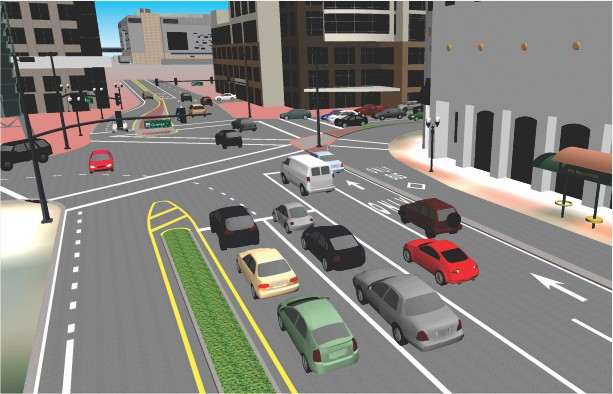
\includegraphics[width=16em,height=9.18em]{eyecatcher.jpg}
}
%%% Title %%%%%%%%%%%%%%%%%%%%%%%%%%%%%%%%%%%%%%%%%%%%%%%%%%%%%%%%%%%%%%%%%%%%%
{\sf\bf
	\\} 
 %%% Authors %%%%%%%%%%%%%%%%%%%%%%%%%%%%%%%%%%%%%%%%%%%%%%%%%%%%%%%%%%%%%%%%%%% 
 { 
 \vspace{0.4em} 
 	{
 		}
}
%%% Logo %%%%%%%%%%%%%%%%%%%%%%%%%%%%%%%%%%%%%%%%%%%%%%%%%%%%%%%%%%%%%%%%%%%%%%
{
% The logos are compressed a bit into a simple box to make them smaller on the result
% (Wasn't able to find any bigger of them.)
\setlength\fboxsep{0pt}
\setlength\fboxrule{0pt}
	\fbox{
		\begin{minipage}{16em}  %distanza dal bordo destro
			\hspace*{2cm}\\ %\includegraphics[scale=0.11]{unict.pdf} \\
		  \hfill \\
		  %\vspace*{-0.6cm}
		  	
\includegraphics[width=16.1em,height=4.95em]{chu-logo.jpg} \\[7ex]
		  	%\includegraphics[width=12em,height=0em]{whitespace.png} \\
			
\includegraphics[width=16em,height=3.38em]{UniversityofCambridgeLogo.png}\\[7ex]
            
\includegraphics[width=16em,height=1.49em]{Complab.png} \\
			%\includegraphics[width=10em,height=4em]{dynanets_logo}
			%\includegraphics[width=4em,height=4em]{aitia_logo}
		\end{minipage}
	}
}
\headerbox{Abstract}{name=section0,span=1,column=0}
 {Nowadays, universities and companies have a huge need for simulation and modelling methodologies. In the particular case of traffic and transportation, making physical modifications to the real traffic networks could be highly expensive, dependent on political decisions and could be highly disruptive to the environment.
However, while studying a specific domain or problem, analysing a problem through simulation may not be trivial and may need several simulation tools, hence raising interoperability issues.
To overcome these problems, we propose an agent-directed transportation simulation platform, through the cloud, by means of services. We intend to use the IEEE standard HLA (High Level Architecture) for simulators interoperability and agents for controlling and coordination. Our motivations are to allow multiresolution analysis of complex domains, to allow experts to collaborate on the analysis of a common problem and to allow co-simulation and synergy of different application domains.
This paper will start by presenting some preliminary background concepts to help better understand the scope of this work. After that, the results of a literature review is shown. Finally, the general architecture of a transportation simulation platform is proposed.

}

\headerbox{Introduction}{name=section1,span=1,column=0,below=section0}
 {Nowadays, universities and companies all around the world have a huge need for simulation and modelling methodologies. The objectives are varied, but simulation is widely used for decision making and what-if analysis, as well as for performance optimisation, testing, training, and so forth. In the particular case of traffic and transportation, making physical modifications to the real traffic networks could be highly expensive, dependent on political decisions and could be highly disruptive to the environment. Therefore, simulation is broadly used in such scenarios.
However, while studying a specific domain or problem, analysing a problem through simulation may not be trivial and very often requires several simulation tools, with different resolutions and domain perspectives, hence raising interoperability issues. Thus instead of helping, simulation could be a headache! Transportation problems usually are complex and fall within this category of problems.
To date, there are not many solutions for traffic that make full use of the intelligent agent concept. However, the multi-agent system metaphor has become recognised as a convenient approach for modelling and simulating complex systems. Also, it has grown enormously not only for being applied to traffic but also to transportation in general terms.
With the recent evolutions in Cloud Computing and Software-as-a-Service (SaaS), there is a new paradigm where simulation software is used in the form of services. Indeed, such evolutions have been more significantly seen in the business world with Information Technology solutions moving to the SaaS paradigm. So, Simulation Software-as-a-Service (SimSaaS) is very beneficial to better exploit the huge amount of platforms and storage that simulation needs \textit{per se} - and Cloud Computing is able to provide such resources. This way, researchers do not need to have the simulation software installed on their own computers or access servers which host this kind of software. Besides, they have new computing environments and methodologies for software development over the Internet.
To address issues arising in this novel perspective the main goal of this paper is to propose an agent-directed transportation simulation platform, through the cloud, by means of services. It is intended to use the IEEE standard HLA (High Level Architecture) for simulators interoperability and agents for controlling and coordination. To do so, it is necessary to build the body of knowledge needed to develop such a platform. This paper's objective is to present the current state of the art in the field and, with that, also to present the general architecture of the intended platform.
The motivations of the platform are to allow multiresolution analysis of complex domains, to allow experts to collaborate on the analysis of a common problem and to allow co-simulation and synergy of different application domains. It is expected to fulfil three main contributions. Firstly, a technological contribution because one will have a cloud-based simulation platform for transportation using HLA and agents where simulations are offered in the form of services. Secondly, a scientific contribution since it will enable the collaboration among experts of the Modelling \& Simulation (M\&S) field with the agent-directed paradigm. Finally, an applied contribution with an agent-oriented platform for scientific simulation, through the cloud, by means of services. Basically, it will be a virtual laboratory.
This paper will start to present some preliminary background concepts regarding M\&S, the agent-oriented paradigm, HLA and cloud for a better understanding of the scope of this work. After that, the results of a literature review concerning SimSaaS in the Cloud, HLA and services, and agent-directed SimSaaS is shown. Finally, the general architecture of a transportation simulation platform is proposed.


}

\headerbox{Preliminary Background}{name=section2,span=1,column=0,below=section1}
 {
}

\headerbox{Literature Review of Cloud SimSaaS}{name=section3,span=1,column=1}
 {
}

\headerbox{A seamlessly integrated transportation simulation platform}{name=section4,span=1,column=1,below=section3}
 {According to the gaps previously found in the literature review, we propose an integrated transportation simulation platform regarding every term (SimSaaS, HLA and Agent-directed simulation), as it will offer simulation in the form of services, using HLA for interoperability of simulators and agents for collaboration. The general architecture of such platform will be similar to the one described in Figure \ref{fig:csim_arch}. The main differences to such architecture is that it will be adapted in order to support HLA in the \textit{Virtual Resources} tier and Agents in the \textit{Cloud Management} tier.
The scientific community needs collaboration in its pursuit of multidisciplinary achievements. This way, scientific community started to make a first sharing approach by creating public repositories of datasets, which are sustainable, shared and ever-evolving. However, there are other roles/stakeholders that would also benefit from such datasets, such as public decision-makers and the industry alike. Nevertheless, while they are all interested in testing their own algorithms/calculations, just the scientific community generally adopts the philosophy of data sharing. Besides data, we also have processes, methods and plans, which are even less commonly shared.
In this multi-stakeholder and multi-resource philosophy, HLA already supports the inclusion of resources because a federate is sufficiently general to consider not only simulators but also databases, data loggers, and other resources. Therefore, the so-acclaimed agent-directed approach could be used to enable collaboration between experts, sharing not only data but also processes. But, why is this interest in sharing? What is the interest in creating this shared community above the cloud? We believe the answer is simple and consists in generating knowledge and innovation.
Simple sharing methodologies are, for example, personal pages in the platform for each researcher with the created models, similar suggested models, integration of models of other researchers and performed simulations with obtained results. Nevertheless, the agent-directed paradigm could bring better options. For example, some researchers have their own legacy tools, which run some complex and less optimised simulations, producing outputs. It would be much better if these tools were implemented in the platform, and it also had the possibility to deploy agents that act on behalf of the researcher, that initialise these tools and even that generate graphics from the resulting output. It would be like an avatar. In practice, these are services that exist in agents: possibility to start and stop everything, make data collection, make data analysis and even pick the output to serve as the input to other tools.
How the researcher can implement and deploy their own agents? The platform itself in the cloud allows that! As well as there is a methodology like HLA to interoperate simulators, there would exist also a design methodology for each researcher to implement his or her own agent/avatar. Each avatar is characterised by the perceptions, actions and operators that could feature. The cognition is decided by the researcher and is expected to implement his or her own expertise. In summary, this is more than just a scientific environment for empirical science. There is the need to be more than that in order to value stakeholders like public decision makers and industry in general, as they could implement their own simulations in the platform.
There are many fields where such a platform can enhance simulations. For instance, cloud computing is becoming increasingly deep-seated in our lives, and Mark Weiser once said ``The most profound technologies are those that disappear. They weave themselves into the fabric of everyday life until they are indistinguishable from it''. Indeed, living labs can be supported by simulation, as the people in these cases would be receiving stimuli from other virtual realities, supported by the platform.
This platform may seem too futuristic but nowadays technological advances have all the proper means that allow its implementation. Firstly, the ones concerning the management and control of the cloud itself. The amount of existing tools in the field is huge, but they are mostly commercial. While looking for alternatives, decision comes mostly between OpenStack (http://www.openstack.org/) and OpenNebula (http://opennebula.org/).
The implementation of HLA's RTI in the cloud is also possible. Again, there are several tools but most of them do not implement the full HLA specification, or have limitations for free use. Here, the choice is easier and falls in the only two tools that seem to be still active, namely the PoRTIco project (http://www.porticoproject.org/) and Pitch pRTI (http://www.pitch.se/).


}

\headerbox{Literature Review of Cloud SimSaaS}{name=section3,span=1,column=2}
 {
}

\headerbox{A seamlessly integrated transportation simulation platform}{name=section4,span=1,column=2,below=section3}
 {According to the gaps previously found in the literature review, we propose an integrated transportation simulation platform regarding every term (SimSaaS, HLA and Agent-directed simulation), as it will offer simulation in the form of services, using HLA for interoperability of simulators and agents for collaboration. The general architecture of such platform will be similar to the one described in Figure \ref{fig:csim_arch}. The main differences to such architecture is that it will be adapted in order to support HLA in the \textit{Virtual Resources} tier and Agents in the \textit{Cloud Management} tier.
The scientific community needs collaboration in its pursuit of multidisciplinary achievements. This way, scientific community started to make a first sharing approach by creating public repositories of datasets, which are sustainable, shared and ever-evolving. However, there are other roles/stakeholders that would also benefit from such datasets, such as public decision-makers and the industry alike. Nevertheless, while they are all interested in testing their own algorithms/calculations, just the scientific community generally adopts the philosophy of data sharing. Besides data, we also have processes, methods and plans, which are even less commonly shared.
In this multi-stakeholder and multi-resource philosophy, HLA already supports the inclusion of resources because a federate is sufficiently general to consider not only simulators but also databases, data loggers, and other resources. Therefore, the so-acclaimed agent-directed approach could be used to enable collaboration between experts, sharing not only data but also processes. But, why is this interest in sharing? What is the interest in creating this shared community above the cloud? We believe the answer is simple and consists in generating knowledge and innovation.
Simple sharing methodologies are, for example, personal pages in the platform for each researcher with the created models, similar suggested models, integration of models of other researchers and performed simulations with obtained results. Nevertheless, the agent-directed paradigm could bring better options. For example, some researchers have their own legacy tools, which run some complex and less optimised simulations, producing outputs. It would be much better if these tools were implemented in the platform, and it also had the possibility to deploy agents that act on behalf of the researcher, that initialise these tools and even that generate graphics from the resulting output. It would be like an avatar. In practice, these are services that exist in agents: possibility to start and stop everything, make data collection, make data analysis and even pick the output to serve as the input to other tools.
How the researcher can implement and deploy their own agents? The platform itself in the cloud allows that! As well as there is a methodology like HLA to interoperate simulators, there would exist also a design methodology for each researcher to implement his or her own agent/avatar. Each avatar is characterised by the perceptions, actions and operators that could feature. The cognition is decided by the researcher and is expected to implement his or her own expertise. In summary, this is more than just a scientific environment for empirical science. There is the need to be more than that in order to value stakeholders like public decision makers and industry in general, as they could implement their own simulations in the platform.
There are many fields where such a platform can enhance simulations. For instance, cloud computing is becoming increasingly deep-seated in our lives, and Mark Weiser once said ``The most profound technologies are those that disappear. They weave themselves into the fabric of everyday life until they are indistinguishable from it''. Indeed, living labs can be supported by simulation, as the people in these cases would be receiving stimuli from other virtual realities, supported by the platform.
This platform may seem too futuristic but nowadays technological advances have all the proper means that allow its implementation. Firstly, the ones concerning the management and control of the cloud itself. The amount of existing tools in the field is huge, but they are mostly commercial. While looking for alternatives, decision comes mostly between OpenStack (http://www.openstack.org/) and OpenNebula (http://opennebula.org/).
The implementation of HLA's RTI in the cloud is also possible. Again, there are several tools but most of them do not implement the full HLA specification, or have limitations for free use. Here, the choice is easier and falls in the only two tools that seem to be still active, namely the PoRTIco project (http://www.porticoproject.org/) and Pitch pRTI (http://www.pitch.se/).


}

\end{poster}
\end{document}